\documentclass[../main.tex]{subfiles}

\newcommand{\cI}{\mathcal{I}}
\begin{document}

\section{Backreaction and quantum corrections}
\label{sec:br}

We proceed to compute planar corrections to the OPE which involve the presence of the backreaction. 
This will complete the determination of the planar limit of the holographically dual chiral algebra.

Since the integrals arising from diagrams this section are slightly more involved, we set up the following notations.
The holomorphic coordinate on $\C^3$ will be $Z = (z , w)$ where $w = (w^1,w^2)$ is a holomorphic coordinate on $\C^2$.
The defect will be located along $w = 0$.
In the formulas below, our convention is that $Z^0 = z$ and $Z^i = w^i$ for $i=1,2$.

Before getting into the main computation of the section, we turn our attention to a simpler example.

\subsection{Warmup: holomorphic Chern--Simons theory}

In this section we compute the effects of a backreaction where the bulk fields have no closed string sector, only an open string part. 
Indeed, consider holomorphic Chern--Simons in the presence of a Kodaira--Spencer field which sources a brane wrapping $N$ $D1$ branes $\C \subset \C^3$. 
The backreaction field is 
\[
\mu_{BR} = \frac{\eps_{ij} \wbar^i \d \wbar^j}{4 \pi^2 \|w\|^4} \partial_z \in \PV^{1,1} (\C^3 \setminus \C) . 
\]
This field satisfies the equation
\beqn\label{eqn:csBR}
\dbar \mu_{BR} \wedge \Omega_{w_i=0} = N \delta_{w_i = 0} \del_z 
\eeqn
where $\delta_{w_i=0}$ is the $\delta$-function supported at $w_i=0$.
This couples to the holomorphic Chern--Simons field by 
\[
S_{BR} = \frac12 \int_{\C^3} \mu_{BR} \vee \op{tr}(A \del A) = \frac12 N \int_{\C^3} A^a \frac{\eps_{ij} \wbar^i \d \wbar^j}{\|w\|^4} \partial_z A^a .
\]
We will denote $\omega = \frac{\eps_{ij} \wbar^i \d \wbar^j}{4 \pi^2\|w\|^4}$ so that the coupling can be written $S_{BR} = \frac{N}{2}
\int_{\C^3} A \omega \del_z A.$

The backreaction coupling has a gauge anomaly even at tree-level.
Indeed, the tree-level gauge variation of $S_{BR}$ is
\[
\int_{\C^3} A^a (\dbar \mu_{BR}) \fc^a = \int_{\C_z} A_{\zbar}^a \partial_z \fc^a .
\]
In order to cancel this gauge anomaly one must introduce an $N$-dependent term in the OPE of the currents $J_a[k,l]$. 
In fact, at tree level only the OPE between currents with $k=l=0$ 
is affected by the tree-level backreaction.
In the presence of the backreaction the currents $J_a[0,0]$ form a Kac--Moody algebra of level $N$
\[
J_a[0,0] (0) J_b [0,0] (z) \simeq f_{ab}^c \frac1z J_c[0,0] + \delta_{ab} N \frac1{z^2} {\rm Id} .
\]
The second term in the OPE is present due the the existence of a tree-level anomaly which involves the back reaction.
The diagram which represents this anomaly is presented in figure \ref{fig:hcstreebr}.

\begin{figure}
	\begin{tikzpicture}	
			\node (A1) at (3,1) {};
			\node (A2) at (3,-1){};

		\node[circle,draw,fill=black]  (V1) at (1.5,0) {}; 
		\draw[decorate]  (V1) --  (A1);
		\draw[decorate] (V1) -- (A2);
		%\draw[decorate,decoration={snake}](0,-1) -- (V2);
		\draw[dashed] (0,0) -- (V1);

		\draw (0,2) -- (0,-2);	
		
	\end{tikzpicture}
	\label{fig:hcstreebr}
	\caption{Tree-level diagram involving the backreaction which contributes an anomaly.}  
\end{figure}

What about higher loop anomalies involving the backreaction?
For scaling dimension reasons, there are no further corrections to the $J_a[0,0]-J_b[0,0]$ OPE.
Let's consider the possibility of quantum corrections to the OPE between the fields $J_a[1,0]$ and $J_b[0,1]$. 
Before accounting for the back reaction, the tree and one-loop level OPE is 
\beqn\label{eqn:Jbr}
J_a[1,0](z) J[0,1]_b \simeq \frac{1}{z} f^c_{ab} J[1,1] + \hbar \frac1z K^{fe} f_{ae}^c f_{bf}^d J_c[0,0] J_d[0,0] ,
\eeqn
see section 6 of \cite{CPkoszul}.
By conformal invariance, the possible $N$-dependent terms in the OPE $J_a[1,0] (0) J_b [0,1](z)$ must be of the form
\[
\alpha f^c_{ae} K^{be}  \left(\frac{1}{z^2} J_c[0,0] + \frac{1}{z} \del_z J_c[0,0] \right) + \beta K^{ab} \frac{1}{z^3} {\rm Id} 
\]
for some (possibly zero) constants $\alpha,\beta$ which depend on~$N$
(notice that the form of the central term in the last term is consistent with the fact that $J[1,0], J[0,1]$ are of spin $3/2$).
The diagrams which give rise to the anomalies necessitating these terms in the OPE are presented in figure \ref{fig:hcsloopbr}.
In these diagrams, the dotted lines represent coupling to the backreaction and the wiggle lines represent bulk propagators.

\begin{figure}
	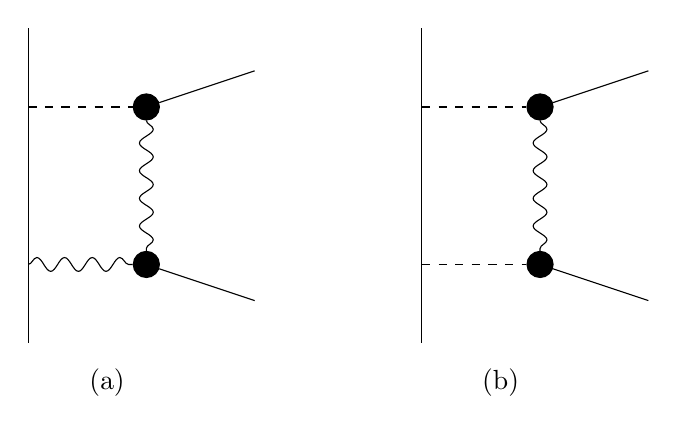
\begin{tikzpicture}
	\begin{scope}		
			\node (A1) at (3,1.5) {};
			\node (A2) at (3,-1.5){};

		\node[circle,draw,fill=black]  (V1) at (1.5,1) {}; 
		\node[circle,draw,fill=black]  (V2) at (1.5,-1) {};  
		\draw[decorate]  (V1) --  (A1);
		\draw[decorate, decoration={snake}] (V1) -- (V2);
		\draw[decorate] (V2) -- (A2);
		\draw[decorate,decoration={snake}](0,-1) -- (V2);
		\draw[dashed] (0,1) -- (V1);

		\draw (0,2) -- (0,-2);	
		
		\node[] at (1,-2.5) {(a)};
		
	\end{scope}

		\begin{scope}[shift={(5,0)}]		
			\node (A1) at (3,1.5) {};
			\node (A2) at (3,-1.5){};

		\node[circle,draw,fill=black]  (V1) at (1.5,1) {}; 
		\node[circle,draw,fill=black]  (V2) at (1.5,-1) {};  
		\draw[decorate]  (V1) --  (A1);
		\draw[decorate, decoration={snake}] (V1) -- (V2);
		\draw[decorate] (V2) -- (A2);
		\draw[dashed](0,-1) -- (V2);
		\draw[dashed] (0,1) -- (V1);

		\draw (0,2) -- (0,-2);	
		
		\node[] at (1,-2.5) {(b)};
	\end{scope}
	\end{tikzpicture}
	\label{fig:hcsloopbr}
	\caption{One-loop diagrams involving the backreaction which contribute an anomaly.}  
\end{figure}

As usual, to evaluate these diagrams we use point splitting on the defect so that operators are placed at $z_1$,$z_2 \in \C$ with $|z_1-z_2| \geq \epsilon$.
The edges of the diagram are labeled by the propagator for the free part of holomorphic Chern--Simons theory is determined by the parametrix for the $\dbar$-operator on $\C^3$:
\beqn
(\dbar P) \wedge \d^3 Z = \delta_{Z=0} .
\eeqn
Explicitly, this is the $(0,2)$-form
\beqn\label{eqn:propagatorCS}
P(Z) = \frac{1}{4 \pi^3 r^6} \ep_{ijk} \br Z^{i} \d \br Z^j \d \br Z^k .
\eeqn

We first focus on diagram \ref{fig:hcsloopbr} (b).
The weight is represented by the integral
\beqn
\int_{(X,Y) \in \C^3_1 \times \C^3_2} A_1(X) \, \omega (x) \,  \del_z \del_w P(X,Y) \, \omega(y) \, A_2(Y) ,
\eeqn
In appendix \ref{appx:hcsbr} we evaluate this integral to obtain
\beqn
\pi N^2 K_{ab} \eps_{ij} \int_{|z_1-z_2| \geq \epsilon} \frac{1}{(z_1 - z_2)^3} \del_{w_i} A^a_1 \del_{w_j} A^b_2 |_{w=0},
\eeqn
where $A_1,A_2$ are the input gauge fields.
The linear BRST variation $A \mapsto A + \dbar c$ of this diagram thus gives rise to the anomaly
\beqn
\pi N^2 K_{ab} \eps_{ij} \int_{|z_1-z_2| \geq \epsilon} \frac{1}{(z_1-z_2)^3} \del_{w_1} A^a \del_{w_2} \dbar c^b |_{w=0}
\eeqn
Integrating by parts and taking $\epsilon \to 0$ this becomes
\beqn
\pi N^2 K_{ab} \eps_{ij} \del^3 \delta_{z_1=z_2} \del_{w_1} A^a \del_{w_2} \dbar c^b |_{w=0} .
\eeqn
In this form it is clear that this anomaly is canceled by introducing the term in the OPE in \eqref{eqn:Jbr} with
\beqn
\beta = \pi N^2 .
\eeqn
\brian{constant is probably wrong}



\subsection{Tree-level backreaction in Kodaira--Spencer theory}

We now turn to the effects of backreaction in our version of Kodaira--Spencer theory obtained by compactifying the twist of type IIB supergravity on a $K3$ surface.
The first nontrivial contribution from the backreaction occurs at tree-level. 
Part of this contribution was computed in \cite{CP}.
The backreaction field $\mu_{BR} = \mu_{BR}(\bfeta)$ takes a similar form as in the previous section.
It is a distributional section
\beqn
\mu_{BR} \in \PV^{1,1}(\C^3) \otimes A
\eeqn
which satisfies the defining distributional equation
\beqn
\dbar \mu_{BR} = \delta_{w_i=0} F \del_z ,
\eeqn
where $F \in H^2(K3) \subset A$ is the flux labeling the brane configuration.

The field $\mu_{BR}$ couples to the fields $\mu_i$ via
\beqn\label{eqn:brmu1mu2}
\int_{Z,\bfeta} \mu_{BR} \mu_1  \mu_2
\eeqn
It couples to the fields $\alpha ,\gamma$ through
\beqn\label{eqn:brag}
\int_{Z,\bfeta} \mu_{BR} \alpha \del_z \gamma .
\eeqn
Notice that by type reasons the backreaction field does not couple to the Beltrami field~$\mu_z$ in the direction parallel to the brane.

We first consider the gauge anomaly involving the coupling \eqref{eqn:brmu1mu2}. 
The tree-level gauge variation of the backreaction coupling \eqref{eqn:brmu1mu2} is
\beqn\label{eqn:brtreeanomaly1}
\int_{Z,\bfeta} \mu_{BR} \dbar \lie{c}_1  \mu_2 +  \int_{Z,\bfeta} \mu_{BR}  \mu_1  \dbar \lie{c}_2 = \int_{z,\bfeta} \left(\lie{c}_1 \mu_2 + \mu_1 \lie{c}_2\right)|_{w = 0} .
\eeqn
Similarly, the tree-level gauge variation of the coupling \eqref{eqn:brag} is 
\beqn\label{eqn:brtreeanomaly2}
\int_{Z,\bfeta} \mu_{BR} \dbar \lie{c}_\alpha  \del_z\gamma  +  \int_{Z,\bfeta} \mu_{BR}  \alpha  \dbar \del_z\lie{c}_\gamma = \int_{z,\bfeta} \left(\lie{c}_\alpha \del_z \gamma + \alpha \del_z\lie{c}_\gamma\right)|_{w = 0} .
\eeqn

Notice that neither of these expression involve $w_i$-derivatives. 
Since $\til{J}^i[0,0]$ couples to $\mu_i$, the anomaly in \eqref{eqn:brtreeanomaly1} can be cancelled by the gauge variation of 
\beqn
\int_{z,\bfeta,z',\bfeta'} \til{J}^1[0,0](z) \mu_1(z) \til{J}^2[0,0] (z') \mu_2(z')
\eeqn
provided that the $\til{J}^i[0,0]$ operators satisfy an appropriate OPE. 
Similarly, the anomaly in \eqref{eqn:brtreeanomaly2} can be cancelled by the gauge variation of a coupling of the form
\beqn
\int_{z,\bfeta,z',\bfeta'} G_\alpha[0,0](z) \alpha(z) G_\gamma[0,0] (z') \gamma (z') .
\eeqn

Proceeding as above by working in the Fourier dual odd coordinates and working with on-shell fields, we see that to cancel the first of these anomalies there must be a term in the $\til J \til J$ OPE of the form
\beqn
\til{J}^i[0,0](0,\what\bfeta) \til{J}^j [0,0] (z,\what\bfeta') \simeq \epsilon^{ij} \frac1z \what F (\what\bfeta + \what\bfeta') .
\eeqn
Using the constraints \eqref{eqn:constraint1} we can write this OPE in terms of on-shell fields as
\beqn
J[1,0](0,\what \bfeta) J[0,1] (z,\what \bfeta') \simeq \frac{1}{z} \what F(\what \bfeta + \what \bfeta') .
\eeqn
To cancel the second anomaly \eqref{eqn:brtreeanomaly2} there must be a term in the $GG$ OPE of the form
\beqn
G_\alpha[0,0](0,\what \bfeta) G_\gamma[0,0](z,\what \bfeta'\\) \simeq \frac1{z^2} \what F (\what \bfeta + \what \bfeta') .
\eeqn

Recall that in section \ref{s:sugraelliptic} we pointed out a discrepancy in our supergravity  elliptic genus and the one computed in \cite{deBoerEG}, which in the notation of that section arose from the two representations $(\frac{\bf 1}{\bf 2})_S \otimes H^{2,0}(K3)$ and $(\frac{\bf 1}{\bf 2})_S \otimes H^{2,2}(K3)$.
We observe that these representations form a sub chiral algebra.
Indeed, if we expand $J[1,0]$ in the Fourier dual coefficients as
\beqn
J[1,0](\what \bfeta) = J_0[1,0] + \what \eta J_{\what \eta} [1,0] + \cdots ,
\eeqn
and similarly for $J[0,1]$, then these representations correspond to the fields 
\beqn
J_0 [1,0],J_{\what \eta}[1,0],J_0 [0,1],J_{\what \eta}[0,1] .
\eeqn
The only OPE's between these fields involves the flux $F$.
They are given by
\begin{align*}
J_0 [1,0](0) J_{\what \eta} [0,1] (z) \simeq \frac{\br f}{z}  \\ 
J_0[0,1] (0) J_{\what \eta} [1,0] (z) \simeq - \frac{\br f}{z} 
\end{align*}
where $\br f$ is the component of $\br \bfeta$ in the original flux $F \in H^2(K3)$.

%As a simple consequence of this, we see that the operators 
%\[
%J[1,0](\what \bfeta), J[0,1](\what \bfeta),G_\alpha[0,0](\what \bfeta), G_\gamma[0,0](\what \bfeta)
%\]
%form a subalgebra of the full gravitational chiral algebra.
%Indeed, the $JG$ OPE's for this class of operators vanish.
%We can relate this to a familiar system of free fields.
%Recall that the spin of the operator $G_\alpha[0,0]$ is one.
%If we choose a spin zero operator $\til G_{\alpha}[0,0]$ such that $\del \til G_\alpha [0,0]$ then we can obtain the same OPE as above if we declare that 
%\beqn
%\til G_\alpha[0,0](0,\what \bfeta) G_\gamma[0,0](z,\what \bfeta') \simeq \frac1{z} \what F (\what \bfeta^a + \what \bfeta'^a) .
%\eeqn
%The operators $J[1,0](\what \bfeta), J[0,1](\what \bfeta),G
%'_\alpha[0,0](\what \bfeta), G_\gamma[0,0](\what \bfeta)$ form a familiar chiral algebra of free fields.
%Explicitly, this is the $\beta \gamma bc$ system valued in 
%\brian{finish, say what the free theory is more explicitly, refer back to CDR.}

\subsection{The propagator for Kodaira--Spencer theory}

In this section we recall the form of the propagator for Kodaira--Spencer theory following \cite{CLbcov1}. 

The propagator for Kodaira--Spencer theory on $\C^3$ is the kernel for the operator $\del \dbar^* \tr^{-1}$. 
We obtain this by applying the divergence operator to the kernel for the operator $\dbar^* \tr^{-1}$ (the analytic part of this kernel is the same as the analytic part of the propagator used in holomorphic Chern--Simons theory). 
%Let us first recall the construction of the kernel for $\dbar^* \tr^{-1}$.

As usual, we use $Z = (Z_1 = w_1, Z_2=w_2,Z_3=z)$ for the holomorphic coordinate on $\C^3$.
Using the Calabi--Yau form one can express the integral kernel for the operator $\dbar^* \tr^{-1}$ in terms of the distributional Kodaira--Spencer field
\beqn
P(Z) = \frac{1}{4 \pi^3 r^6} \ep_{ijk} \br Z^{i} \d \br Z^j \d \br Z^k \del^3,
\eeqn
where $\del^3 = \del_{Z_1} \del_{Z_2} \del_{Z_3}$.
%This is a smooth section of $\PV^{3,2}(\C^3)$ away from $0 \in \C^3$.
The kernel is obtained by pulling back this section along the difference map 
\[
\C^3 \times \C^3 \to \C^3,\quad (Z,Z') \mapsto Z - Z' .
\]
We denote the pulled back section by
\[
P(Z,Z') \in \br{\PV}^{3,2}(\C^3 \times \C^3) . 
\]
Here $\br{\PV}^{3,2}$ stands for distributional Dolbeault valued polyvector fields of type $(3,2)$.
Notice that this section is smooth away from the diagonal in $\C^3 \times \C^3$. 

We are interested in the Kodaira--Spencer propagator which we will denote by $\bf P$; this is the kernel of the operator $\del \dbar^* \triangle^{-1}$. 
To obtain this, we first apply the divergence operator to $P$ 
\[
\bP = \del P \in \br\PV^{2,2}(\C^3) .
\]
Explicitly this is
\beqn
\bP (Z) = \frac{3}{4 \pi^3 r^8} \ep_{ijk} \ep_{lmn} \br Z^{i} \br Z^l \d \br Z^j \d \br Z^k \del_{Z_m} \del_{Z_n} .
\eeqn
%\begin{align*}
%P(z,w_i) = & \pm \frac{\d \wbar_1 \d \wbar_2}{r^8} \left(\zbar^2 \partial_{w_1} \partial_{w_2} - \zbar w_1 \partial_z \partial_{w_2} + \zbar w_2 \partial_z \partial_{w_1} \right) \\ 
%& \pm \frac{\d \wbar_2 \d \zbar}{r^8} \left(\zbar \wbar_1 \partial_{w_1} \partial_{w_2} - \wbar_1^2 \partial_z \partial_{w_2} + \wbar_1 \wbar_2 \partial_z \partial_{w_1}\right) \\
%& \pm \frac{\d \zbar \d \wbar_1}{r^8} \left(\zbar \wbar_2 \partial_{w_1} \partial_{w_2} - \wbar_1 \wbar_2 \partial_z \partial_{w_2} + \wbar_2^2 \partial_z \partial_{w_1} \right) .
%\end{align*}
Pulling back along the difference map we obtain the Kodaira--Spencer theory propagator
\[
\bP (Z,Z') \in \br\PV^{2,2}(\C^3 \times \C^3) .
\]
This distribution is the integral kernel for the operator $\partial \dbar^* \tr^{-1}$ acting on poyvector fields. 
As in the case of the propagator for holomorphic Chern--Simons theory it is a smooth away from the diagonal. 
We interpret this propagator as a symmetric element of the (completed) tensor square of the fields of Kodaira--Spencer theory on~$\C^3$. 

The propagator for Kodaira--Spencer theory on $K3 \times \C^3$ (after compactification) is the kernel for the operator $\partial \dbar^* \tr^{-1}$ acting on the full space of fields which acts on the odd $\bfeta$-coordinates by the identity:
\beqn
\bP(Z, \bfeta ; Z, \bfeta') = \bP(Z,Z') \delta_{\bfeta = \bfeta'} .
\eeqn

\subsection{The order $N$ term} 
\label{sec:oneloop}

\begin{figure}
	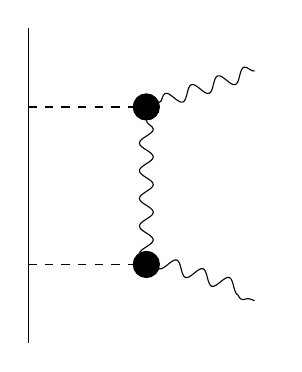
\begin{tikzpicture}

		\begin{scope}		
			\node (A1) at (3,1.5) {};
			\node (A2) at (3,-1.5){};

		\node[circle,draw,fill=black]  (V1) at (1.5,1) {}; 
		\node[circle,draw,fill=black]  (V2) at (1.5,-1) {};  
		\draw[decorate, decoration={snake}]  (V1) --  (A1);
		\draw[decorate, decoration={snake}] (V1) -- (V2) -- (A2);
		\draw[dashed](0,-1) -- (V2);
		\draw[dashed] (0,1) -- (V1);

		\draw (0,2) -- (0,-2);	
	\end{scope}
	\end{tikzpicture}
	\label{fig:orderN}
	\caption{The order $N$ term.}  
\end{figure}

In this section we compute the anomaly associated to the diagram \ref{fig:orderN} which involves two backreaction vertices and a single propagator.
We first consider the terms in the backreaction coupling involving the fields $\mu_1,\mu_2$.
The weight of this diagram involving these fields is represented by the integral
\beqn
\int_{X,\bfeta_X, Y, \bfeta_Y} \mu_1(X) \, \mu_{BR} (x) \,  \bP (X,Y) \, \mu_{BR}(y) \, \mu_2(Y) ,
\eeqn


\subsection{The order $N^{1/2}$ term}


%\section{Superconformal algebra}
%
%\begin{itemize}
%\item The bosonic operator $T = T^0 [0,0]|_{\bfeta = 0}$ is the stress energy tensor in the superconformal algebra. 
%\item The bosonic operators $J [r,s]|_{\bfeta = 0}$, for $r + s = 2$ comprise the $SU(2)_R$ current.
%Denote $J_0 = J [1,1]|_{\bfeta = 0}$, $J_+ = J^0 [2,0]|_{\bfeta = 0}$, $J_- = J^0[0,2]|_{\bfeta = 0}$. 
%\item The fermionic elements of the superconformal algebra are given by the pair of $SU(2)_R$ doublets 
%\[
%\begin{pmatrix} G_+ \\ \Bar{G}_+ \end{pmatrix} = \begin{pmatrix} \sqrt{2} G^0_\alpha [1,0]|_{\bfeta = 0} \\ \sqrt{2} G^0_\gamma [1,0]|_{\bfeta = 0} \end{pmatrix} , \quad \begin{pmatrix} G_- \\ \Bar{G}_- \end{pmatrix} = \begin{pmatrix} \sqrt{2} G^0_\alpha [0,1]|_{\bfeta = 0} \\ \sqrt{2} G^0_\gamma [0,1]|_{\bfeta = 0} \end{pmatrix}
%\]
%\end{itemize}
%
%
%\subsection{The $TT$ OPE}
%
%In Section \ref{sec:TT1} we computed the tree-level $TT$ OPE at the level of general $w$-descendants.
%Specializing just to $T (z) = T^0[0,0](z)$ we find that the tree-level OPE becomes the usual charge zero Virasoro OPE
%\[
%T(0) T(z) \simeq 2 \frac{1}{z^2} T(0) + \frac{1}{z} \partial_z T(0) .
%\]
%
%At the quantum level, this OPE is deformed. 
%In \S \ref{sec:oneloop} we have shown that there is a one-loop correction to the $\til J \til J$ OPE of the form 
%\[
%\til J^{1}[1,0] (0, \what\bfeta = 0) \til J^{2} [0,1] (z, \what\bfeta'=0) |_{\text{1-loop}} \simeq \frac{N^2}{z^2} .
%\]
%Now, since 
%\[
%T[0,0] (\bfeta) = \til T[0,0] (\bfeta) - \frac12 \left(\del_z \til J^{1}[1,0] (\bfeta) - \del_z \til J^{2}[0,1] (\bfeta) \right) 
%\]
%we see that 
%\[
%T(0) T(z)|_{\text{1-loop}} \simeq \# \del_z^2 \frac{N^2}{z^2} = \# \frac{N^2}{z^4} .
%\]
%
%Here, we note that for type reasons, there is no one-loop quantum correction to the $\til T \til T$ OPE so that the the tree-level plus one-loop $TT$ OPE reads
%\[
%T(0) T(z) \simeq \# \frac{N^2}{z^4} + 2 \frac{1}{z^2} T(0) + \frac{1}{z} \partial_z T(0) .
%\]
%
%
%\subsection{The $JJ$ OPE } 
%
%From \eqref{eqn:TJtree} and we see that the $SU(2)$ currents $J_0, J_\pm$ are weight one primary operators
%\[
%T(0) J_\pm (z) \simeq \frac1z \partial_z J_\pm (0) + \frac{1}{z^2} J_\pm (0) 
%\]
%and similarly for $J_0$. 

\section{Acknowledgments}

We are grateful to V. Fernandez, ... for helpful discussions and comments. NP is supported by funds from the Department of Physics and the College of Arts \& Sciences at the University of Washington, the DOE Early Career Research Program under award DE-SC0022924, and the Simons Foundation as part of the Simons Collaboration in Celestial Holography. She also thanks the Perimeter Institute's Visiting Fellow program for additional support and hospitality while this work was underway. Research at Perimeter Institute is supported by the Government of Canada through Industry Canada and by the Province of Ontario through the Ministry of Research and Innovation.
\end{document}
